\scanpage{61}

\mspage{2}

Le même résultat, \inserted{en remplacant $\dim\operatorname{proj}$ par $\operatorname{Tor}\dim$} est encore valable pour $M$ de type fini sur un anneau \deleted{\unsure{local $B$|local N|local}} noethérien $B$, qui soit une $A$-algèbre telle que $mB\subset\operatorname{radical}(B)$

Il faut savoir\quad (i) qu'on peut encore définir la profondeur de $M$ sur $A$ dans ce cas

(ii) que la Tor dimension de $M$ est le plus grand entier $d$ tel que $\operatorname{Tor}^d(k,M)\ne0$, où $k$ est le corps résiduel de $A$.

C'est là une conséquence facile du résultat suivant, pour lequel je ne connais pas de référence :

\uline{prop} : Soit $A$ un anneau \uline{local noethérien}, $\deleted{\unsure{A}}B$ une $A$-algèbre locale noethérienne ($A\longrightarrow B$ étant local), \uline{$m$ un idéal de $A$}, \uline{$\deleted{M}N$ un $A$-module de type fini}, \uline{$M$ un $\deleted{A}B$-module de type fini}. On a

\[
\underline{\varprojlim\operatorname{Tor}^{p}_{A}(N/_{m^kN},M)=
\operatorname{Tor}^{p}_{A}(N,M)^{\wedge}}\qquad\text{et plus précisément}
\]

une égalité de proobjets

\[
\text{``}\varprojlim\text{''}\ \operatorname{Tor}^{p}_{A}(N,M)\big/_{m^k\operatorname{Tor}^{p}(N,\unsure{M|N})}
\xrightarrow{\sim}\ \text{``}\varprojlim\text{''}\ \operatorname{Tor}^{p}_{A}(N/_{m^kN},M)
\]

Si $B$ était plat sur $A$, on prendrait une résolution de $\deleted{\unsure{N}}M$ sur $B$, et il suffirait d'appliquer Artin-Rees, qui exprime que ``le pro-objet complétion'' est foncteur exact. On peut par ailleurs remplacer $B$ par une algèbre dont il soit quotient. On peut aussi compléter $B$. L'assertion résulte alors du lemme suivant, qui coiffe

$0_{\overline{\underline{\mathrm{IV}}}}$ 19.7.1.3\\
et\\
$0_{\overline{\underline{\mathrm{III}}}}$ 10.3.1

\uline{prop} : Soit $A\longrightarrow B$ un homomorphisme local d'\uline{anneaux locaux noethériens}, avec \uuline{$B$ complet}. $B$ est quotient d'un $A$anneau $C$, tel que

% slanted
\margin{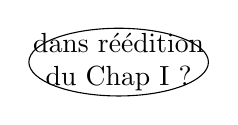
\begin{tikzpicture}[baseline]\node[align=center,inner sep=2pt] (m) {dans réédition\\du Chap I ?};\draw (m.center) ellipse (1.14cm and .43cm);\end{tikzpicture}}

(i) $C$ est local, $A\longrightarrow C$ et et $C\longrightarrow B$ sont locaux

(ii) \uline{$C$ est plat sur $A$}

(iii) Si $k$ est le corps résiduel de $A$, $C_0=C\otimes_A k$, $B_0=B\otimes_A k$, \uline{$C_0$ est un anneau \deleted{de séries formelles sur une extension $K$ de $k$}}\inserted{ régulier}, et l'application graduée associée à $C_0\longrightarrow B_0$ : $\operatorname{gr}C_0\longrightarrow\operatorname{gr}B_0$ est bijective en degré $0$ et $1$

\uline{Démonstration} : Soit $m$ ($n$) l'idéal maximal de $A$ ($B$), $K$ le corps résiduel de $B$.

Soit $t_i$ une base d'un supplémentaire de l'image de $m/_{m^2}\otimes_k K\longrightarrow n/_{n^2}$. Si on relève les $t_i$ dans $B$, on définit une flèche $A[[T_i]]\longrightarrow B$. Soit $A'=A[[T_i]]$, $m'$ son idéal maximal, $A'$ est plat sur $A$, et on a \deleted{\unsure{$m'/m'^2$}}

\[
m'/_{m'^2+mA'}\xrightarrow{\sim} n/_{n^2+mB}.
\]
% archive sheet number: 60
